%%% Класс документа
\documentclass[a4paper,14pt]{article}

%%% Работа с русским языком
\usepackage{cmap}					% поиск в PDF
\usepackage[warn]{mathtext}
\usepackage[T2A]{fontenc}			% кодировка
\usepackage[utf8]{inputenc}			% кодировка исходного текста
\usepackage[english,russian]{babel}	% локализация и переносы
\usepackage{mathtext} 				% русские буквы в формулах
\usepackage{csvsimple}              % for tabular from csv loading
\usepackage{indentfirst}            % indent after sections
%\usepackage{minipage}

%%% Дополнительная работа с математикой
\usepackage{amsmath,amsfonts,amssymb,amsthm,mathtools} % AMS
\usepackage{icomma} % "Умная" запятая: $0,2$ --- число, $0, 2$ --- перечисление

%%% Номера формул
%\mathtoolsset{showonlyrefs=true} % Показывать номера только у тех формул, на которые есть \eqref{} в тексте.
%\usepackage{leqno} % Немуреация формул слева

%%% Шрифты
\usepackage{euscript}	 % Шрифт Евклид
\usepackage{mathrsfs} % Красивый матшрифт

%%% Свои команды
\DeclareMathOperator{\sgn}{\mathop{sgn}}

%%% Перенос знаков в формулах (по Львовскому)
\newcommand*{\hm}[1]{#1\nobreak\discretionary{}
{\hbox{$\mathsurround=0pt #1$}}{}}

%%% Работа с картинками
\usepackage{graphicx}  % Для вставки рисунков
\graphicspath{{images/}{images2/}}  % папки с картинками
\setlength\fboxsep{3pt} % Отступ рамки \fbox{} от рисунка
\setlength\fboxrule{1pt} % Толщина линий рамки \fbox{}
\usepackage{wrapfig} % Обтекание рисунков и таблиц текстом

%%% Работа с таблицами
\usepackage{array,tabularx,tabulary,booktabs} % Дополнительная работа с таблицами
\usepackage{longtable}  % Длинные таблицы
\usepackage{multirow} % Слияние строк в таблице

%%% Теоремы
\theoremstyle{plain} % Это стиль по умолчанию, его можно не переопределять.
%\newtheorem{theorem}{Теорема}[section]
%\newtheorem{proposition}[theorem]{Утверждение}
 
%\theoremstyle{definition} % "Определение"
%\newtheorem{corollary}{Следствие}[theorem]
%\newtheorem{problem}{Задача}[section]
 
%\theoremstyle{remark} % "Примечание"
%\newtheorem*{nonum}{Решение}

%%% Программирование
\usepackage{etoolbox} % логические операторы

%%% Страница
\usepackage{extsizes} % Возможность сделать 14-й шрифт
\usepackage{geometry} % Простой способ задавать поля
	\geometry{top=25mm}
	\geometry{bottom=35mm}
	\geometry{left=35mm}
	\geometry{right=20mm}
	
%%% Колонтитулы
%\usepackage{fancyhdr}
 	%\pagestyle{fancy}
 	%\renewcommand{\headrulewidth}{0mm}  % Толщина линейки, отчеркивающей верхний колонтитул
 	%\lfoot{Нижний левый}
 	%\rfoot{Нижний правый}
 	%\rhead{Верхний правый}
 	%\chead{Верхний в центре}
 	%\lhead{Верхний левый}
 	% \cfoot{Нижний в центре} % По умолчанию здесь номер страницы
 	
%%% Интерлиньяж
%\usepackage{setspace}
%\onehalfspacing % Интерлиньяж 1.5
%\doublespacing % Интерлиньяж 2
%\singlespacing % Интерлиньяж 1

%%% Гиперссылки
\usepackage{hyperref}
\usepackage[usenames,dvipsnames,svgnames,table,rgb]{xcolor}
\hypersetup{				% Гиперссылки
    unicode=true,           % русские буквы в раздела PDF
    pdftitle={Заголовок},   % Заголовок
    pdfauthor={Автор},      % Автор
    pdfsubject={Тема},      % Тема
    pdfcreator={Создатель}, % Создатель
    pdfproducer={Производитель}, % Производитель
    pdfkeywords={keyword1} {key2} {key3}, % Ключевые слова
    colorlinks=true,       	% false: ссылки в рамках; true: цветные ссылки
    linkcolor=red,          % внутренние ссылки
    citecolor=green,        % на библиографию
    filecolor=magenta,      % на файлы
    urlcolor=cyan           % на URL
}

%%% Другие пакеты
\usepackage{lastpage} % Узнать, сколько всего страниц в документе.
\usepackage{soul} % Модификаторы начертания
\usepackage{csquotes} % Еще инструменты для ссылок
%\usepackage[style=authoryear,maxcitenames=2,backend=biber,sorting=nty]{biblatex}
\usepackage{multicol} % Несколько колонок
\usepackage{multirow} % Несколько строк

%%% Шрифты
%\renewcommand{\familydefault}{\sfdefault} % Начертание шрифта


%%% Работа с библиографией
%\usepackage{cite} % Работа с библиографией
%\usepackage[superscript]{cite} % Ссылки в верхних индексах
%\usepackage[nocompress]{cite} % 
%\usepackage{csquotes} % Еще инструменты для ссылок


%%% Tikz
\usepackage{tikz} % Работа с графикой
\usepackage{pgfplots} % Работа с pgf
\usepackage{pgfplotstable}
\usepackage{upgreek}

%%% Дополнительные пакеты для tikz
%\usepgfplotslibrary{dateplot} % Возможность подписания дат
\pgfplotsset{compat=1.5}


\begin{document}

\newcommand{\HRule}{\rule{\linewidth}{0.7mm}} % Defines a new command for the horizontal lines, change thickness here
	
	\begin{center}
		\large\textbf{Московский Физико-Технический Институт}\\ % Name of your university/college
		\large\textbf{(государственный университет)}
	
		\vfill
		
		\Large Лабораторная работа по курсу общей физики № *labnum*\\[0.5cm] % Preambule of your document title
		
		
		\HRule
		\\[0.4cm]
		{ \huge \bfseries *name of your labwork*}% Title of your document
		\\[0.4cm] 
		\HRule
		\\[0.5cm]
		
		\ \\
	\textbf{\large Автор:} \\	
	\large *your name* *groupname*\\ % Your name and something more, your group num for example
		\vfill
		\hspace*{-0.8 cm}
\includegraphics[width=100 pt]{frkt_logo}\\ % logo of your  company/university/college
		\large Долгопрудный, 2021 % location and year
	\end{center}

\newpage
\setcounter{page}{2}
\fancyfoot[c]{\thepage}
\fancyhead[L] {Работа № *labnum*} % some information in page header
\fancyhead[R]{}

\paragraph*{Цель работы:} изучение петель гистерезиса ферромагнитных материалов с помощью осциллографа.

\paragraph*{Оборудование:} автотрансформатор, понижающий трансформатор, амперметр и вольтметр (мультиметры), резистор, делитель напряжения, интегрирующая
цепочка, электронный осциллогра, тороидальные образцы с двумя обмотками..

\section{Теоретическое введение}

\begin{wrapfigure}{l}{0.6\textwidth}
	\vspace{-20pt}
	\begin{center}
		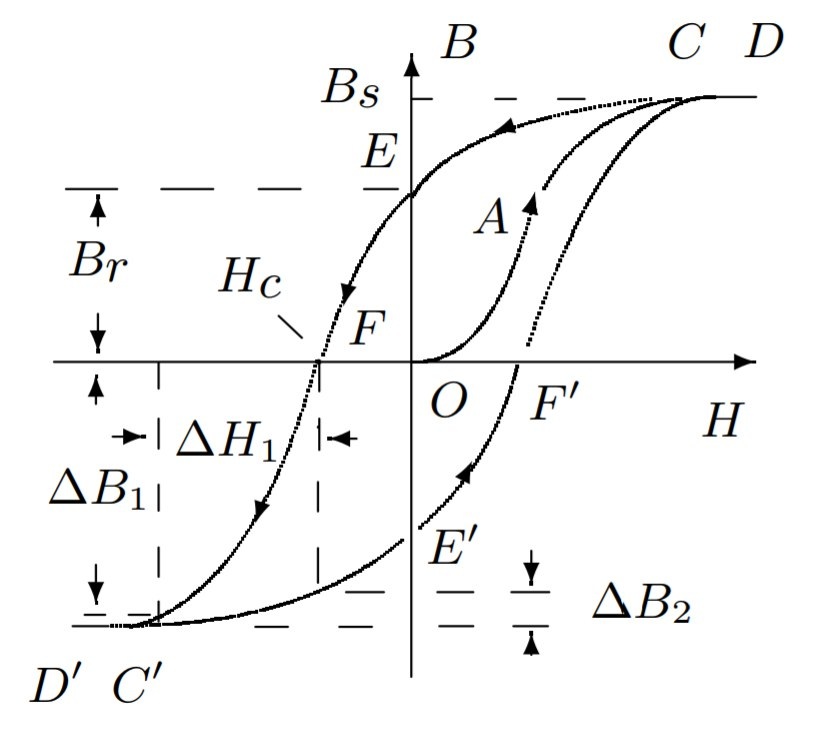
\includegraphics[width=0.7\linewidth]{Image_1.jpeg}
		\label{fig:sdfsafd}
	\end{center}
	\vspace{-10pt}
	\caption{Петля гистерезиса ферромагнетика}
\end{wrapfigure}

Магнитная индукция $\vec{B}$ и напряженность магнитного поля
$\vec{H}$ в ферромагнитном материале неоднозначно связаны
между собой: индукция зависит не только от напряженности, но
и от предыстории образца. Связь между индукцией
и напряженностью поля типичного ферромагнетика иллюстрирует рис. 1. Если
к размагниченному образцу начинают прикладывать магнитное поле, то его намагничивание следует кривой $ OACD $, выходящей
из начала
координат. Эту кривую называют \textit{основной кривой намагничивания}.


Индукция $\vec{B}$ в образце состоит из индукции, связанной с намагничивающим полем
$\vec{B}$, и индукции, создаваемой самим намагниченным
образцом.
В системе СИ эта связь имеет вид

$$\vec{B} = \mu_{0}(\vec{H}+\vec{M}),$$

где $\vec{M}$- \textit{намагниченность} - магнитный момент единичного объема образца, а $\mu_{0}$ - магнитная постоянная.

Намагнитим образец до насыщения - до точки D. Соответствующее
значение индукции $B_{s}$ называют индукцией насыщения. При уменьшении поля $H$ до нуля зависимость $B(H)$ имеет вид кривой $DCE$, и при нулевом поле индукция имеет конечное ненулевое значение. Это остаточная индукция $B_{r}$ . Чтобы размагнитить образец, то есть перевести его в состояние
$F$, необходимо приложить "обратное" магнитное
поле $H_{c}$, которое называют коэрцитивной силой.

Замкнутая кривая $DEFD'E'F'D$, возникающая при циклическом
перемагничивании образца, намагниченного до насыщения, называется \textit{предельной петлей гистерезиса.}


\subsection{Измерение магнитной индукции в образцах.}
Магнитную индукцию удобно определять с помощью ЭДС, возникающей при изменении магнитного потока Ф в катушке, намотанной на образец:

$$\mathscr{E} = -\dfrac{dФ}{dt}.$$

Тогда отсюда и из формулы $Ф=BSN_{и}$ получаем:
$$|B|=\dfrac{1}{SN_{и}}\int \mathscr{E}dt.$$
Для интегрирования сигнала применяют интегрирующие схемы (рис. 2).

\begin{wrapfigure}{l}{0.6\textwidth}
	\vspace{-20pt}
	\begin{center}
		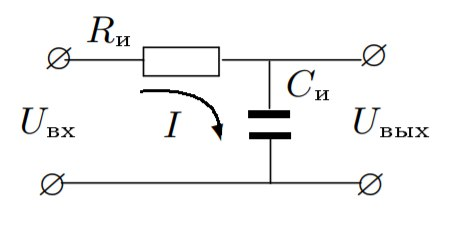
\includegraphics[width=0.7\linewidth]{Image_2.jpeg}
		\label{fig:sdfsafd}
	\end{center}
	\vspace{-10pt}
	\caption{Интегрирующая RC-цепь}
\end{wrapfigure}

Если выходной сигнал намного меньше входного ($U_{вых}\ll U_{вх},$) ток в цепи пропорционален входному напряжению: $I\simeq\dfrac{U_{вх}}{R}$, а напряжение на емкости С

$$U_{вых}\simeq\dfrac{1}{RС}\int U_{вх}dt.$$

Этот вывод тем ближе к истине, чем больше постоянная $\tau=RC$ превосходит характерное время процесса (например, его период). Для синусоидальных напряжений

$$U_{вых}=\dfrac{U_{вх}}{RC\Omega},$$

где $\Omega$ - частота сигнала.

В итоге, обозначив параметры интегрирующей цепи через $R_{и}$ и $C_{и}$, получаем

$$ |B|=\dfrac{1}{SN_{и}}\int U_{вх}dt=\dfrac{R_{и}С_{и}}{SN_{и}}U_{вых}.$$

\section{Экспериментальная установка.}
Схема экспериментальной установки показана на рис. 3.

Действующее значение переменного тока в обмотке N0 измеряется амперметром А (мультиметром GDM). Последовательно с амперметром включено сопротивление $R_{0}$, напряжение с которого подается на вход X электронного осциллографа (ЭО). Это напряжение пропорционально току в обмотке $N_{0}$, а следовательно и напряженности H магнитного поля в образце.

Для измерения магнитной индукции B с измерительной обмотки $N_{И}$ на вход интегрирующей RC -цепочки подается напряжение $U_{И}$ (UВХ), пропорциональное производной $\dot{B}$, а с выхода снимается напряжение $U_{C}$($U_{ВЫХ}$), пропорциональное
величине B , и подается на вход Y осциллограа.
Замкнутая кривая, возникающая на экране, воспроизводит в некотором масштабе (различном для осей X и Y ) петлю гистерезиса. Чтобы придать этой кривой количественный смысл, необходимо установить масштабы изображения, т.е. провести калибровку каналов X и Y ЭО. Для этого, во-первых, надо узнать, каким напряжениям (или токам) соответствуют амплитуды сигналов, видимых на экране, и во-вторых,  каким значениям B и H соответствуют эти напряжения
(или токи).

\newpage

\begin{figure}[h!]
	\centering
	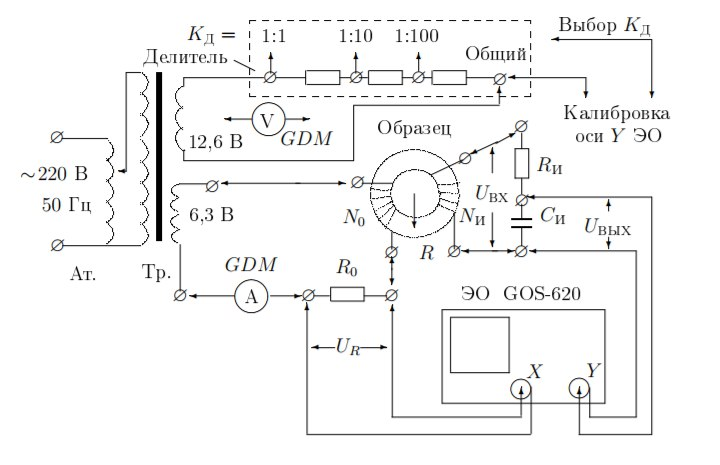
\includegraphics[width=\linewidth]{Image_3.jpeg}
	\caption{Схема установки для исследования намагничивания образцов}
	\label{fig:Holl2}
\end{figure}

\newpage

\section{Обработка данных}

Эксперементальные данные собираем с трех образцов: феррита, пермаллоя (Fe-Ni) и кремнистого железа (Fe-Si).
Для каждого из изучаемых образцов определим, при каких значениях тока и напряжения на осцилографе наблюдается предельная петля.
После этого снимем зависимость тока и напряжения.

Для расчета напряженности магнитного поля воспользуемся формулой

\begin{equation}
	H = \frac{I N_0}{2 \pi r}
\end{equation}

где $r$ -- радиус тороидального соленоида, $N_0$ -- количество витков в первичной обмотке.

Индукцию магнитного поля найдем по формуле

\begin{equation}
	B = \frac{R C U}{S N_u}
\end{equation}

где $R$, $C$ -- параметры $RC$-цепи, $N_u$ -- количество витков во вторичной обмотке.
По полученным данным построим графики зависимости $B(H)$, а так же найдем $\mu$ вещества

\begin{equation}
	\mu = \frac{B}{\mu_0 H}
\end{equation}

где $\mu_0 = 4 \pi \cdot 10^{-7}$.
Отметим, что поскольку мы используем цепь переменного тока, вольметр и амперметр дают на выходе
эффективные значение напряжения и силы тока. Для того, чтобы получить амплитудные значения,
необходимо выходные значения умножить на $\sqrt{2}$.

\begin{equation}
	U = \sqrt{2} U_{\text{эф}} ~~
	I = \sqrt{2} I_{\text{эф}}
\end{equation}

\subsection{Образец 1 (феррит)}

Запишем параметры образца:

\begin{center}
	$N_0 = 35$                 \\
	$N_u = 400$                \\
	$S = 3 ~ \text{см}^2$      \\
	$2 \pi r = 25 ~ \text{см}$
\end{center}

Предельная петля наблюдается при 

\begin{center}
	$I = 132,38 ~ \text{мА}$ \\
	$U = 36,62 ~ \text{мВ}$
\end{center}

\begin{figure}[h!]
	\centering
	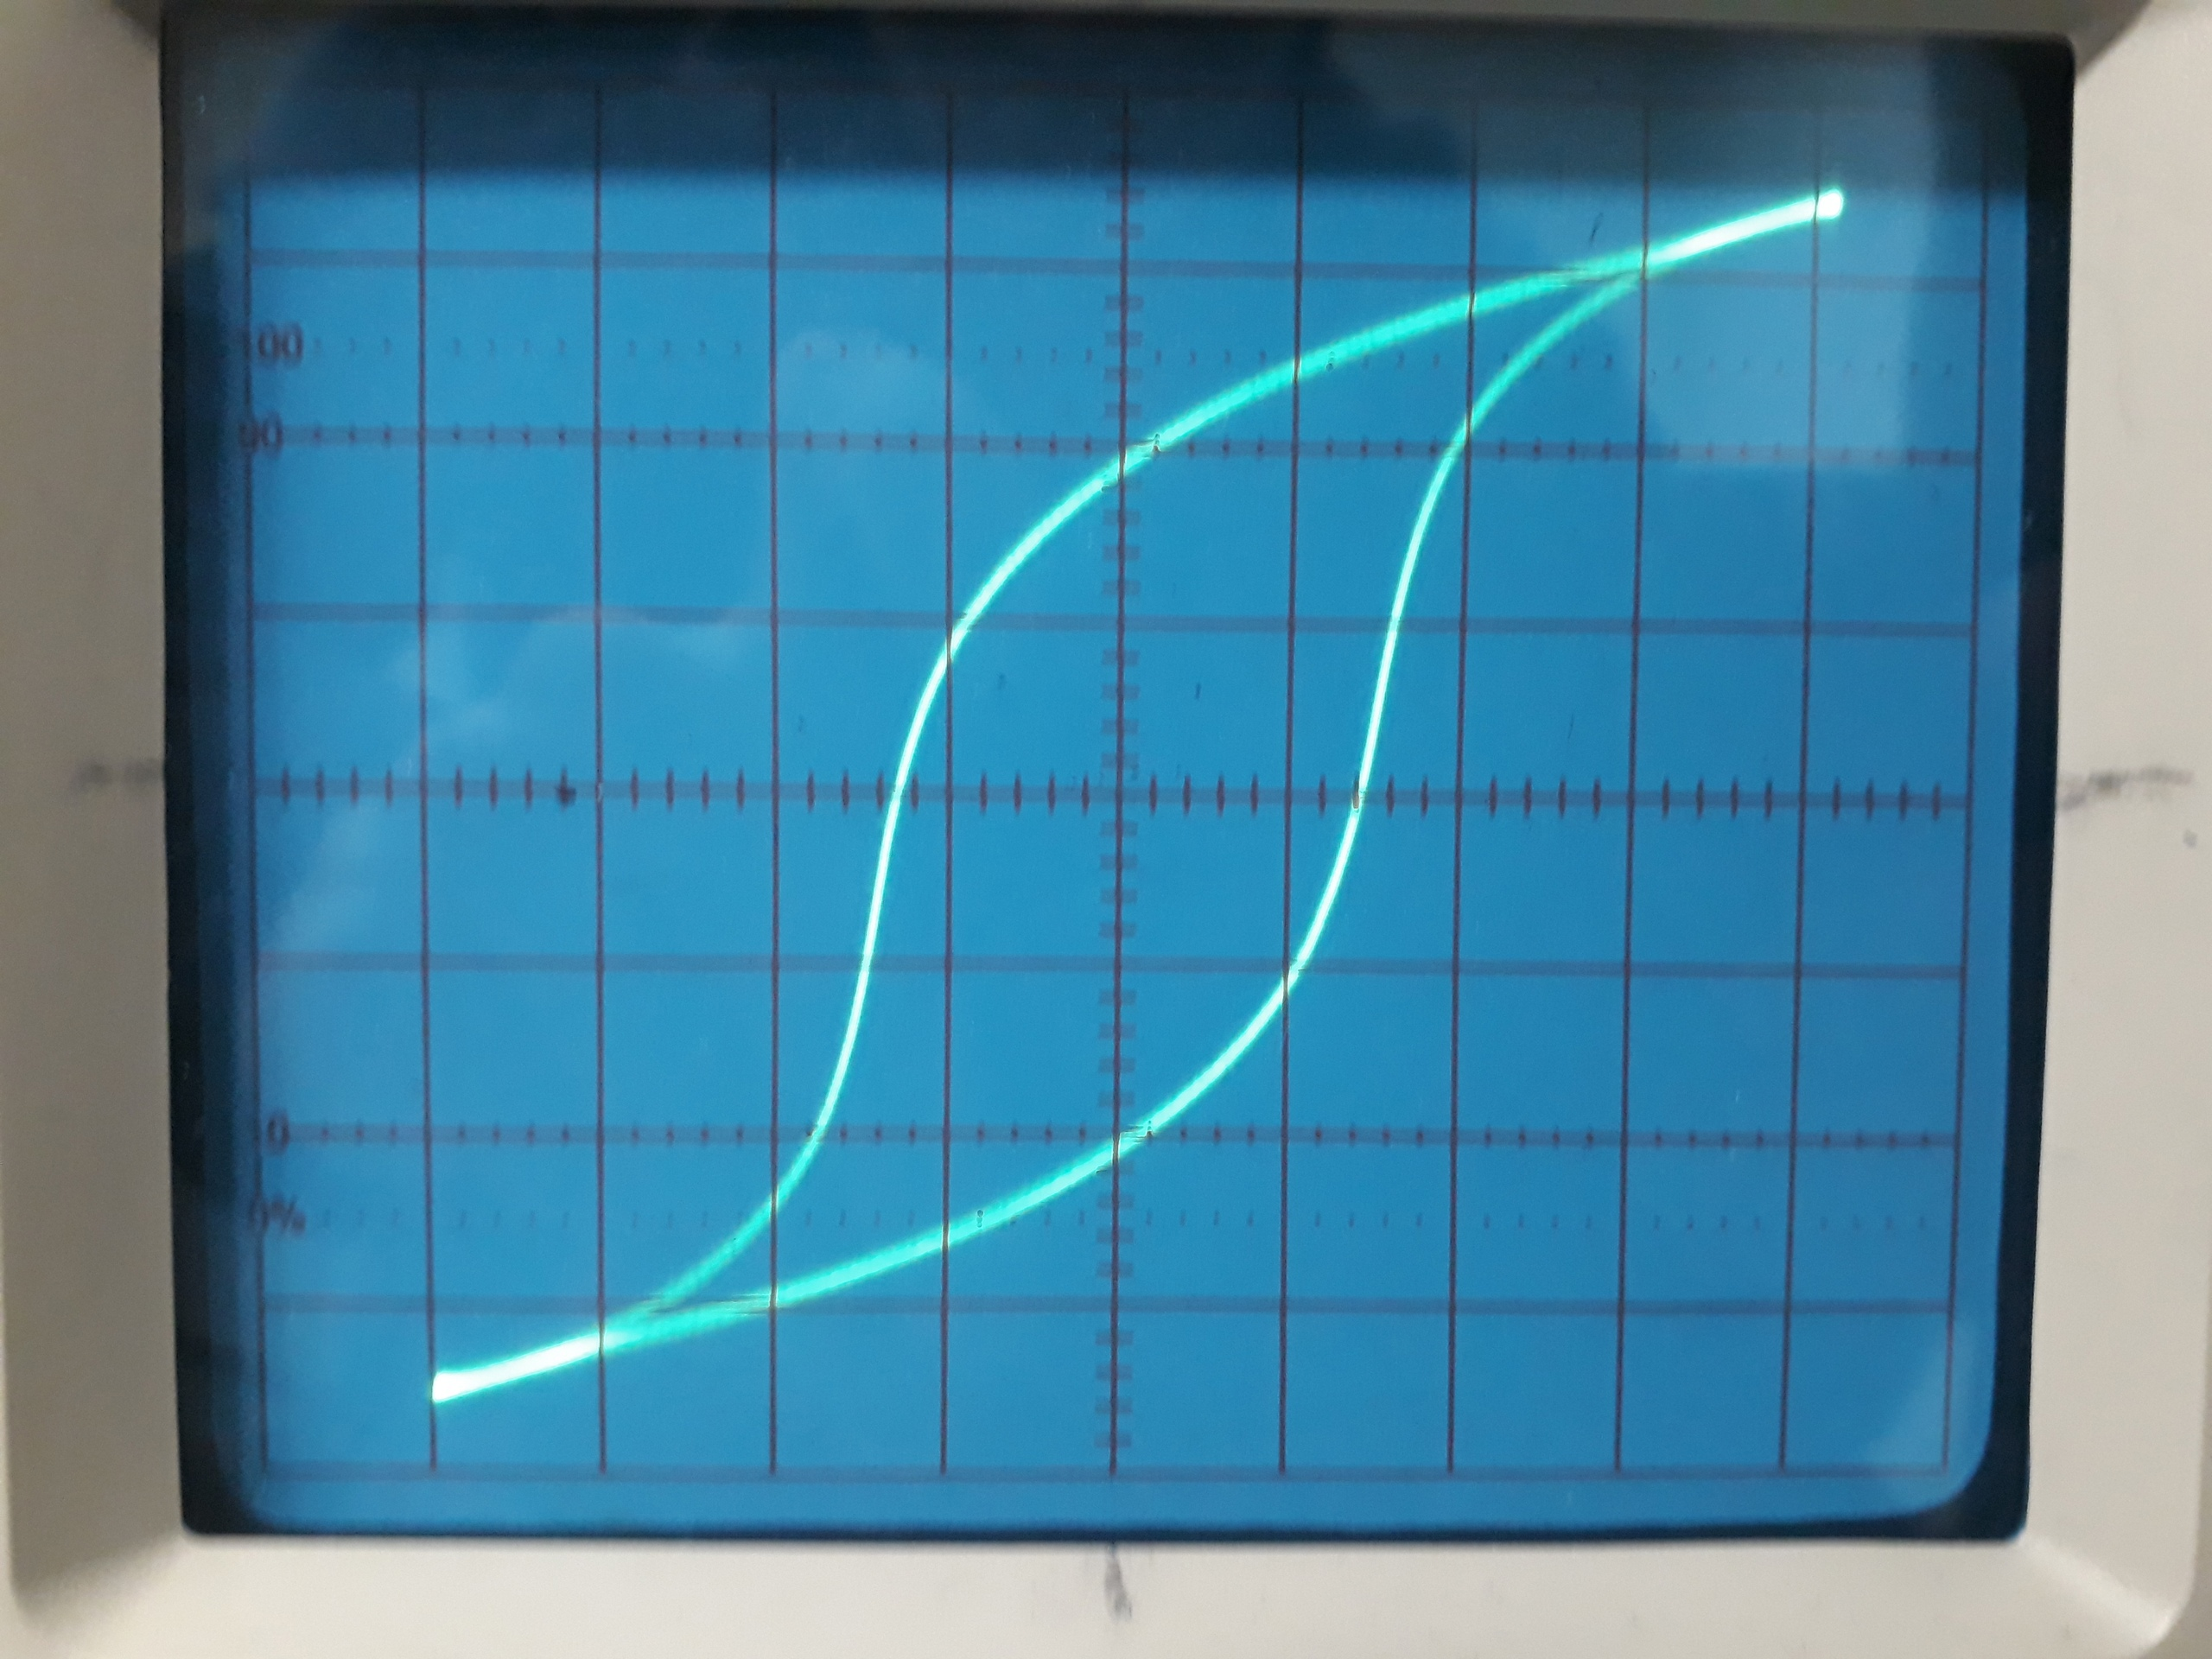
\includegraphics[width=0.7\linewidth]{sample1.jpg}
	\caption{Предельная петля, феррит}
	\label{sample1_pic}
\end{figure}

\begin{figure}
	\centering
	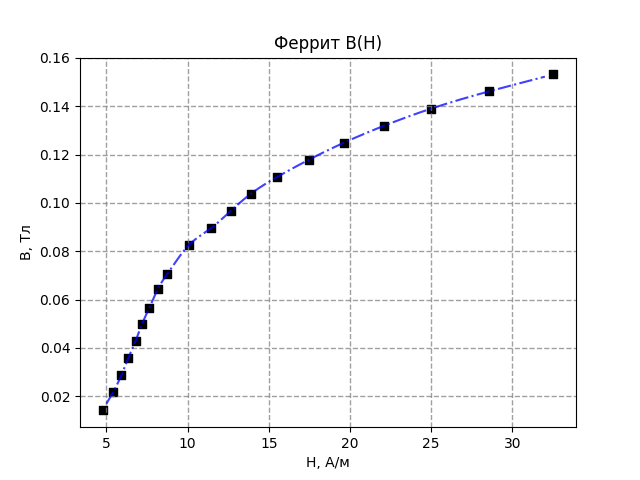
\includegraphics[width=0.7\linewidth]{sample1_B(H)Python.png}
	\caption{Феррит, график зависимости $B(H)$}
	\label{sample1_BH}
\end{figure}

\begin{figure}
	\centering
	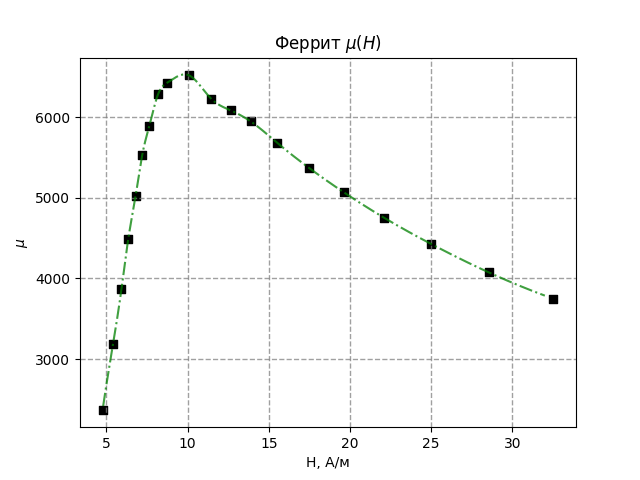
\includegraphics[width=0.7\linewidth]{sample1_mu(H)Python.png}
	\caption{Феррит, график зависимости $\mu(H)$}
	\label{sample1_muH}
\end{figure}

\newpage

\begin{table}[h!]
    \begin{center}
        \begin{tabular}{|c|c|c|c|c|c|c|}
            \hline
            $I_{\text{эф}}$, мА  & $I$, мА   & $H$, А/м  & $U_{\text{эф}}$, мВ  & $U$, мВ  & $B$, Тл & $\mu$      \\ \hline
            24,05                & 34,01     & 4,76      & 3,00                 & 4,24     & 0,01    & 2 363,46   \\ \hline
            27,33                & 38,65     & 5,41      & 4,60                 & 6,51     & 0,02    & 3 189,04   \\ \hline
            29,92                & 42,31     & 5,92      & 6,10                 & 8,63     & 0,03    & 3 862,86   \\ \hline
            32,06                & 45,34     & 6,35      & 7,60                 & 10,75    & 0,04    & 4 491,50   \\ \hline
            34,33                & 48,55     & 6,80      & 9,10                 & 12,87    & 0,04    & 5 022,37   \\ \hline
            36,36                & 51,42     & 7,20      & 10,60                & 14,99    & 0,05    & 5 523,61   \\ \hline
            38,60                & 54,59     & 7,64      & 12,00                & 16,97    & 0,06    & 5 890,27   \\ \hline
            41,32                & 58,44     & 8,18      & 13,70                & 19,37    & 0,06    & 6 282,05   \\ \hline
            44,22                & 62,54     & 8,76      & 15,00                & 21,21    & 0,07    & 6 427,08   \\ \hline
            50,87                & 71,94     & 10,07     & 17,50                & 24,75    & 0,08    & 6 518,05   \\ \hline
            57,80                & 81,74     & 11,44     & 19,00                & 26,87    & 0,09    & 6 228,26   \\ \hline
            63,85                & 90,30     & 12,64     & 20,50                & 28,99    & 0,10    & 6 083,23   \\ \hline
            70,10                & 99,14     & 13,88     & 22,00                & 31,11    & 0,10    & 5 946,29   \\ \hline
            78,40                & 110,87    & 15,52     & 23,50                & 33,23    & 0,11    & 5 679,28   \\ \hline
            88,17                & 124,69    & 17,46     & 25,00                & 35,36    & 0,12    & 5 372,30   \\ \hline
            99,10                & 140,15    & 19,62     & 26,50                & 37,48    & 0,12    & 5 066,56   \\ \hline
            111,70               & 157,97    & 22,12     & 28,00                & 39,60    & 0,13    & 4 749,48   \\ \hline
            126,30               & 178,62    & 25,01     & 29,50                & 41,72    & 0,14    & 4 425,47   \\ \hline
            144,15               & 203,86    & 28,54     & 31,00                & 43,84    & 0,15    & 4 074,63   \\ \hline
            164,30               & 232,36    & 32,53     & 32,50                & 45,96    & 0,15    & 3 747,89   \\ \hline
        \end{tabular}
    \end{center}
    \caption{Феррит}
	\label{sample1_table}
\end{table}

По результатам эксперемента максимальное значение магнитной проницаемости
для феррита $\mu_{max} = 6518$

\begin{center}
	\fbox{$H_c = 9,0$ А/м; $B_s = 13,3$ Тл}
\end{center}

\subsection{Образец 2 (пермаллой)}

Запишем параметры образца:

\begin{center}
	$N_0 = 40$                   \\
	$N_u = 200$                  \\
	$S = 3,8 ~ \text{см}^2$      \\
	$2 \pi r = 24 ~ \text{см}$
\end{center}

Предельная петля наблюдается при 

\begin{center}
	$I = 233,54 ~ \text{мА}$ \\
	$U = 169,28 ~ \text{мВ}$
\end{center}

\newpage

\begin{figure}[h!]
	\centering
	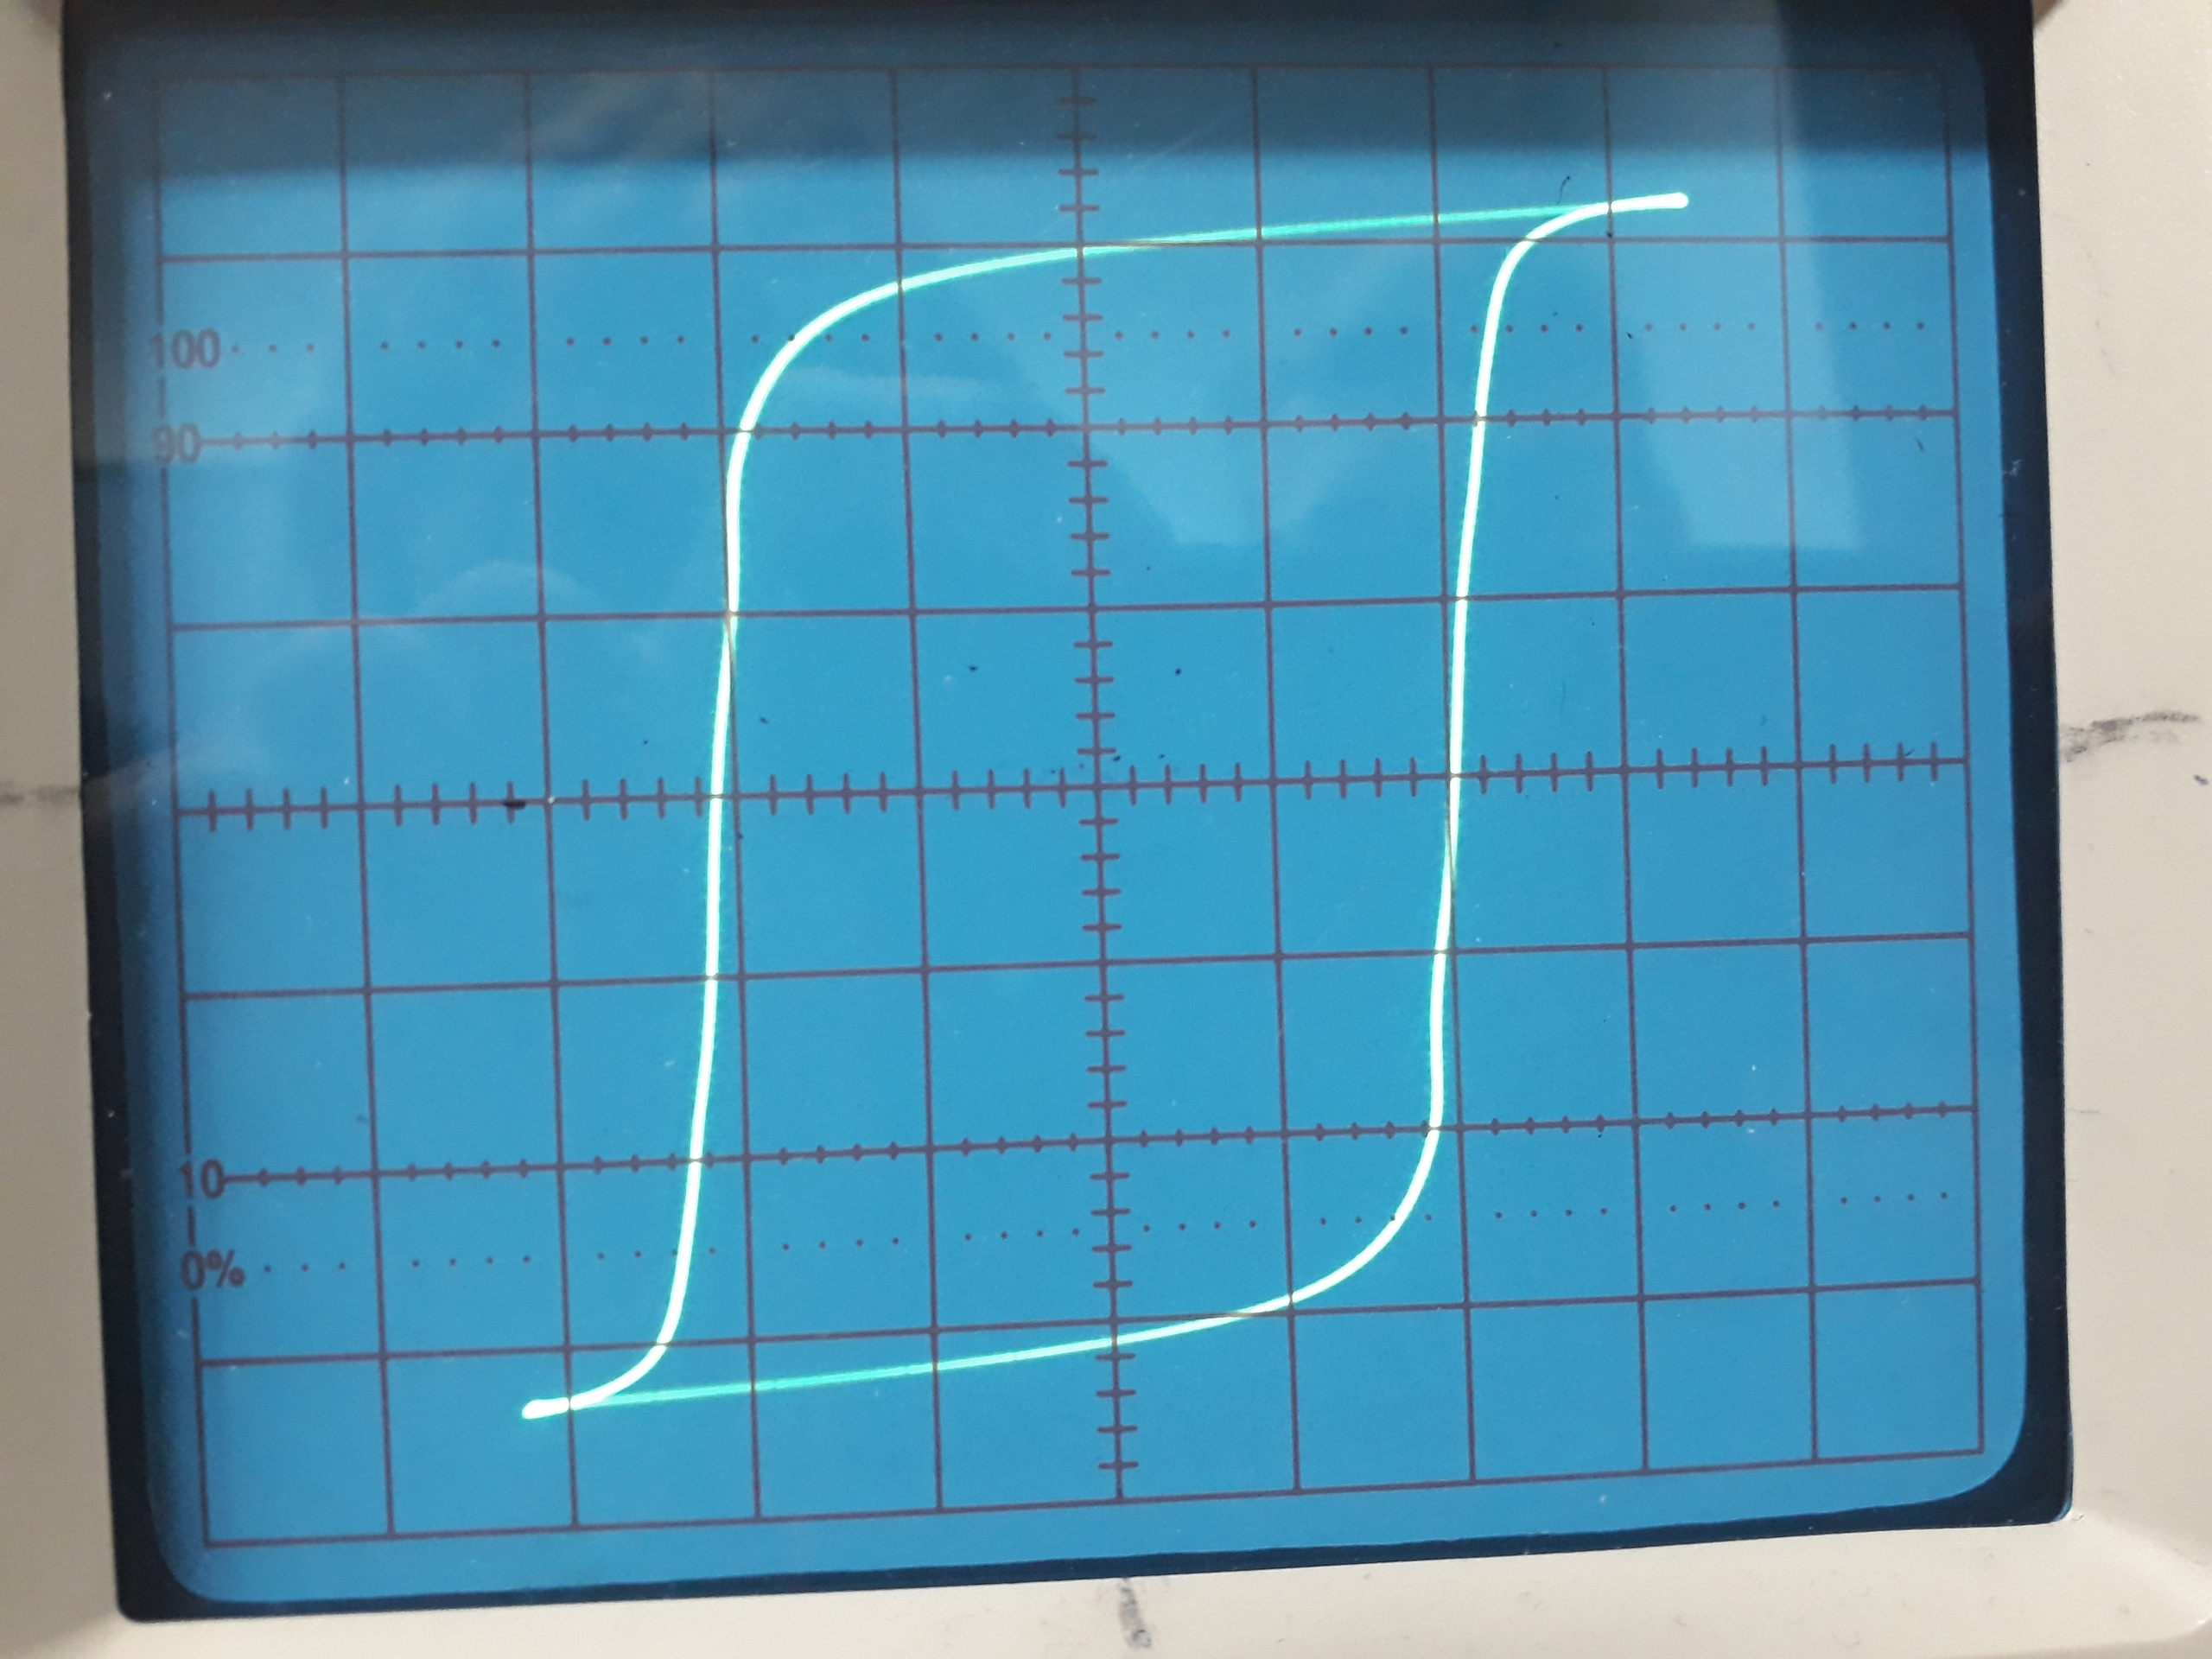
\includegraphics[width=0.7\linewidth]{sample2.jpg}
	\caption{Предельная петля, пермаллой}
	\label{sample2_pic}
\end{figure}

\begin{figure}
	\centering
	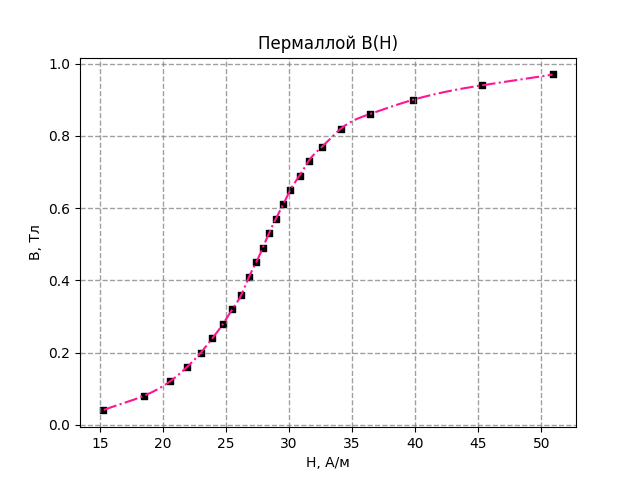
\includegraphics[width=0.7\linewidth]{sample2_B(H)Python.png}
	\caption{Пермаллой, график зависимости $B(H)$}
	\label{sample2_BH}
\end{figure}

\begin{figure}
	\centering
	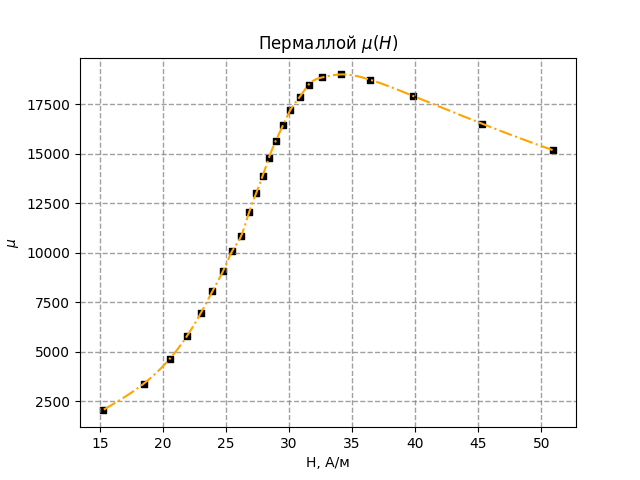
\includegraphics[width=0.7\linewidth]{sample2_mu(H)Python.png}
	\caption{Пермаллой, график зависимости $\mu(H)$}
	\label{sample2_muH}
\end{figure}

\newpage

\begin{table}[h!]
    \begin{center}
        \begin{tabular}{|c|c|c|c|c|c|c|}
            \hline
            $I_{\text{эф}}$, мА  & $I$, мА   & $H$, А/м  & $U_{\text{эф}}$, мВ  & $U$, мВ  & $B$, Тл & $\mu$      \\ \hline
            64,50                & 91,22     & 15,20     & 5,20                 & 7,35     & 0,04    & 2 025,96   \\ \hline
            78,28                & 110,70    & 18,45     & 10,50                & 14,85    & 0,08    & 3 370,75   \\ \hline
            87,16                & 123,26    & 20,54     & 16,10                & 22,77    & 0,12    & 4 641,91   \\ \hline
            92,90                & 131,38    & 21,90     & 21,40                & 30,26    & 0,16    & 5 788,77   \\ \hline
            97,60                & 138,03    & 23,00     & 27,00                & 38,18    & 0,20    & 6 951,88   \\ \hline
            101,49               & 143,53    & 23,92     & 32,50                & 45,96    & 0,24    & 8 047,26   \\ \hline
            105,10               & 148,63    & 24,77     & 38,00                & 53,74    & 0,28    & 9 085,92   \\ \hline
            108,20               & 153,02    & 25,50     & 43,50                & 61,52    & 0,32    & 10 103,00  \\ \hline
            111,20               & 157,26    & 26,21     & 48,10                & 68,02    & 0,36    & 10 869,97  \\ \hline
            113,77               & 160,90    & 26,82     & 54,50                & 77,07    & 0,41    & 12 038,07  \\ \hline
            116,22               & 164,36    & 27,39     & 60,20                & 85,14    & 0,45    & 13 016,79  \\ \hline
            118,40               & 167,44    & 27,91     & 65,50                & 92,63    & 0,49    & 13 902,01  \\ \hline
            120,50               & 170,41    & 28,40     & 71,00                & 100,41   & 0,53    & 14 806,74  \\ \hline
            122,80               & 173,67    & 28,94     & 76,50                & 108,19   & 0,57    & 15 654,93  \\ \hline
            125,28               & 177,17    & 29,53     & 82,10                & 116,11   & 0,61    & 16 468,33  \\ \hline
            127,66               & 180,54    & 30,09     & 87,40                & 123,60   & 0,65    & 17 204,61  \\ \hline
            130,80               & 184,98    & 30,83     & 93,00                & 131,52   & 0,69    & 17 867,48  \\ \hline
            133,83               & 189,26    & 31,54     & 98,50                & 139,30   & 0,73    & 18 495,71  \\ \hline
            138,40               & 195,73    & 32,62     & 103,90               & 146,94   & 0,77    & 18 865,47  \\ \hline
            144,70               & 204,64    & 34,11     & 109,50               & 154,86   & 0,82    & 19 016,64  \\ \hline
            154,34               & 218,27    & 36,38     & 115,20               & 162,92   & 0,86    & 18 756,95  \\ \hline
            169,10               & 239,14    & 39,86     & 120,60               & 170,55   & 0,90    & 17 922,22  \\ \hline
            192,30               & 271,95    & 45,33     & 126,40               & 178,76   & 0,94    & 16 517,94  \\ \hline
            216,24               & 305,81    & 50,97     & 130,60               & 184,70   & 0,97    & 15 177,33  \\ \hline
            \end{tabular}
    \end{center}
    \caption{Пермаллой}
	\label{sample2_table}
\end{table}

По результатам эксперемента максимальное значение магнитной проницаемости
для пермаллоя $\mu_{max} = 19016$

\begin{center}
	\fbox{$H_c = 19,2$ А/м; $B_s = 1,2$ Тл}
\end{center}

\subsection{Образец 3 (кремнистое железо)}

Запишем параметры образца:

\begin{center}
	$N_0 = 35$                   \\
	$N_u = 350$                  \\
	$S = 1,2 ~ \text{см}^2$      \\
	$2 \pi r = 10 ~ \text{см}$
\end{center}

Предельная петля наблюдается при 

\begin{center}
	$I = 877,38 ~ \text{мА}$ \\
	$U = 167,44 ~ \text{мВ}$
\end{center}

\begin{figure}
	\centering
	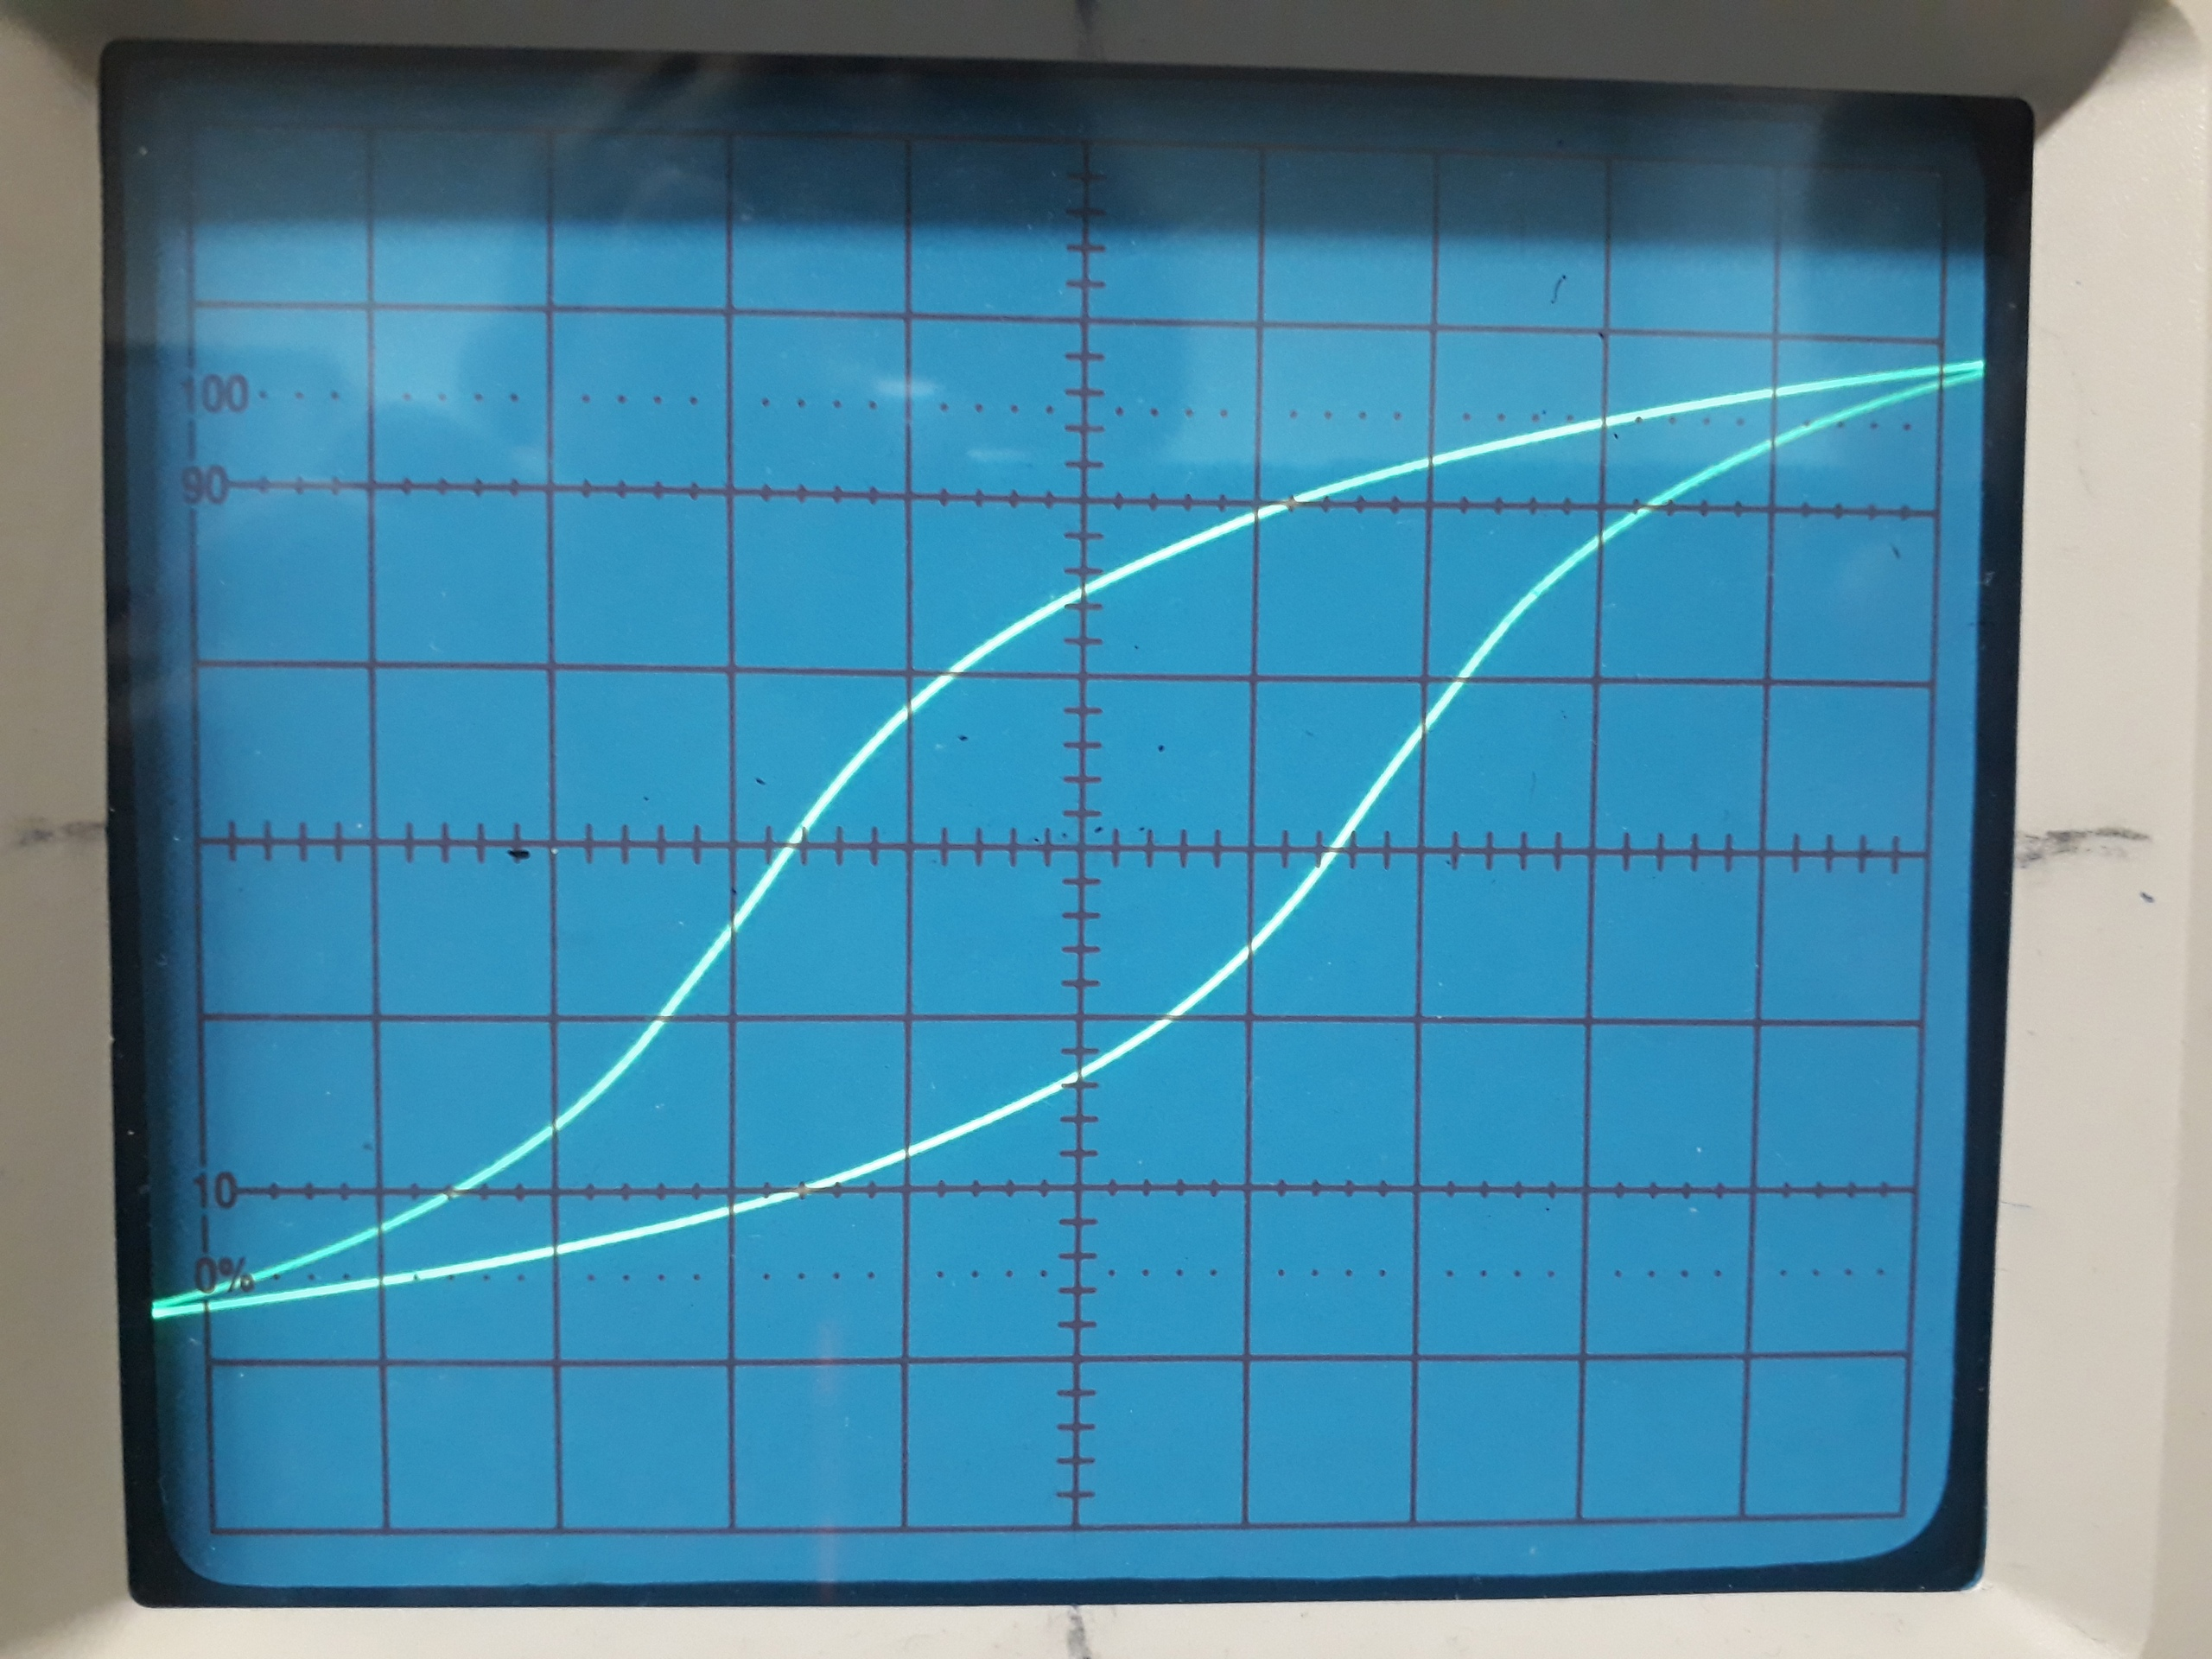
\includegraphics[width=0.7\linewidth]{sample3.jpg}
	\caption{Предельная петля, кремнистое железо}
	\label{sample3_pic}	
\end{figure}

\section{Вывод}

Петля гистерезиса является качественной характеристикой намагничивания ферромагнетика, 
показывая такие эффекты, как домены, в том числе площадь петли пропорциональна энергии, 
теряемой в единице объёма вещества за время цикла.

\section{Дополнительные вопросы к работе}

\begin{enumerate}
	\item Вывести формулу индуктивности тора $L$ (длинного соленоида) с магнитным сердечником. 
	Рассчитать $L$ для первичной и вторичной обмоток.

	\begin{figure}
		\centering
		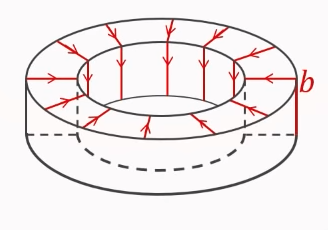
\includegraphics[width=0.7\linewidth]{Тороидальная катушка.png}
		\caption{Тороидальная катушка}
		% \label{}
	\end{figure}

	Пусть есть тороидальная катушка с внутренним радиусом $R$ и числом витков $N$. По теореме о циркуляции
     
    \begin{equation}
        B \cdot 2 \pi r = \frac{4 \pi}{c} I \Rightarrow B = \frac{2 \mu N}{cr} I
    \end{equation}
    
    Тогда поток вектора индукции через тороидальную катушку прямоугольного сечения
    
    \begin{equation}
        \int_R^{R+a} B(r) N b dr = \int_R^{R+a} \frac{2 \mu N^2}{cr} I b dr = \frac{2 \mu N^2 I b}{c} \ln \frac{R + a}{R} 
    \end{equation}
    
    \begin{equation}
        \Phi = \frac{2 \mu N^2 I b}{c} \ln \frac{R + a}{R} = \frac{L I}{c}
    \end{equation}
    
    Тогда индуктивность тороидальной катушки
    
    \begin{equation}
        L = 2 \mu N^2 b \ln \frac{R + a}{R}
    \end{equation}
    
    Если проволака намотана тонким радиусом, то выполняется соотношение $\frac{a}{R} \ll 1$. 
	В этом случае, раскладывая натуральный логарифм в ряд Тейлора получим \footnote{В данной задаче мы считали,
	что тороидальная катушка имеет прямоугольное сечение с площадью $S$, указанной в параметрах образца, поэтому получим расчетную формулу
	$L = \frac{2 \mu N^2 S}{R}$}
    
    %% в общем-то, вместо a, b в этой формуле можно подставить r^2, где r -- радиус намотки
    \begin{equation}
        L = \frac{2 \mu N^2 b a}{R}
    \end{equation}
    %% после этого в общем-то все величины становятся известными, и можно вычислить индуктивность для первичной и вторичной обмоток

	\begin{table}[h!]
    \begin{center}
        \begin{tabular}{|c|c|c|}
            \hline
                        & первичная обмотка $L_0$, мГн & вторичная обмотка $L_u$, мГн \\ \hline
            феррит      & 12,03                        & 1572,18                      \\ \hline
            пермаллой   & 60,53                        & 1513,32                      \\ \hline
        \end{tabular}
    \end{center}
    \caption{индуктивность}
\end{table}

	\item Определить резонансную частоту контура на вторичной обмотке. Оценить его добротность.
	
	Согласно схеме, мы имеем дело с параллельным RCL-контуром. Выражение для резонансной частоты
    
	Параметры установки: $R_u = 200$ кОм, $C = 200$ мкФ.

	%% L -- расчитываем из пункта 1, C -- дано в схеме
	\begin{equation}
		\omega_0 = \frac{1}{\sqrt{LC}}
	\end{equation}

	Резонансная частота на феррите $\omega_0 = 56,39 ~ \text{с}^{-1}$.
	Резонансная частота на пермаллое $\omega_0 = 57,49 ~ \text{с}^{-1}$.
	
	Добротность для последовательного контура
	
	\begin{equation}
		Q = R \sqrt{\frac{C}{L}}
	\end{equation}

	Добротность контура при исследовании феррита:
	
	\begin{center}
		\fbox{$Q = 71,4$ }	
	\end{center}

	Добротность контура при исследовании пермаллоя:
	
	\begin{center}
		\fbox{$Q = 72,8$ }	
	\end{center}

	\item Определить реактивные сопротивления катушки, емкости и сравнить их с активным сопротивлением.

	%% не понятно, какую частоту контура брать. Возможно резонансную
	\begin{equation}
		X_L = \omega L ~ X_C = \frac{1}{\omega C}
	\end{equation}

	Значения реактивных сопративлений для феррита: $X_L = 280,2$ Ом, $X_C = 280,1$ Ом;

	Значения реактивных сопративлений для пермаллоя: $X_L = 274,8$ Ом, $X_C = 274,7$ Ом;

	Активное сопративление схемы $R = 200000$ Ом. Можем убедиться в том, что
	для обоих образцов $X_L \ll R$ и $X_C \ll R$.

	\item Пояснить качественно, как будет меняться резонансная частота контура в зависимости от тока через первичную обмотку.
	
	При небольших токах вклад в общий поток, а с ним собственно и
	в индуктивность, дает как магнитное поле, создаваемое током, так и
	намагниченность сердечника.

	При достаточно больших токах последнее слагаемое перестает вносить вклад, так как существует состояние насыщения. Следовательно,
	при достаточно больших токах при его увеличении общая индуктивность
	падает, а так как $\omega = \frac{1}{\sqrt{LC}}$, то резонансная частота возрастает.

\end{enumerate}

\end{document}